\documentclass{beamer}
\usepackage{amsmath}
\usepackage[english]{babel} %set language; note: after changing this, you need to delete all auxiliary files to recompile
\usepackage[utf8]{inputenc} %define file encoding; latin1 is the other often used option
\usepackage{csquotes} % provides context sensitive quotation facilities
\usepackage{graphicx} %allows for inserting figures
\usepackage{booktabs} % for table formatting without vertical lines
\usepackage{textcomp} % allow for example using the Euro sign with \texteuro
\usepackage{stackengine}
\usepackage{wasysym}
\usepackage{tikzsymbols}
\usepackage{textcomp}
% ELIMINAR COMANDOS DE NAVEGACION%%%%%%%%%%%
\setbeamertemplate{navigation symbols}

%\newcommand{\bubblethis}[2]{
 %       \tikz[remember picture,baseline]{\node[anchor=base,inner sep=0,outer sep=0]%
 %       (#1) {\underline{#1}};\node[overlay,cloud callout,callout relative pointer={(0.2cm,-0.7cm)},%
 %       aspect=2.5,fill=yellow!90] at ($(#1.north)+(-0.5cm,1.6cm)$) {#2};}%
 %   }%
%\tikzset{face/.style={shape=circle,minimum size=4ex,shading=radial,outer sep=0pt,
 %       inner color=white!50!yellow,outer color= yellow!70!orange}}

%% Some commands to make the code easier
\newcommand{\emoticon}[1][]{%
  \node[face,#1] (emoticon) {};
  %% The eyes are fixed.
  \draw[fill=white] (-1ex,0ex) ..controls (-0.5ex,0.2ex)and(0.5ex,0.2ex)..
        (1ex,0.0ex) ..controls ( 1.5ex,1.5ex)and( 0.2ex,1.7ex)..
        (0ex,0.4ex) ..controls (-0.2ex,1.7ex)and(-1.5ex,1.5ex)..
        (-1ex,0ex)--cycle;}
\newcommand{\pupils}{
  %% standard pupils
  \fill[shift={(0.5ex,0.5ex)},rotate=80] 
       (0,0) ellipse (0.3ex and 0.15ex);
  \fill[shift={(-0.5ex,0.5ex)},rotate=100] 
       (0,0) ellipse (0.3ex and 0.15ex);}

\newcommand{\emoticonname}[1]{
  \node[below=1ex of emoticon,font=\footnotesize,
        minimum width=4cm]{#1};}
\usepackage{scalerel}
\usetikzlibrary{positioning}
\usepackage{xcolor,amssymb}
\newcommand\dangersignb[1][2ex]{%
  \scaleto{\stackengine{0.3pt}{\scalebox{1.1}[.9]{%
  \color{red}$\blacktriangle$}}{\tiny\bfseries !}{O}{c}{F}{F}{L}}{#1}%
}
\newcommand\dangersignw[1][2ex]{%
  \scaleto{\stackengine{0.3pt}{\scalebox{1.1}[.9]{%
  \color{red}$\blacktriangle$}}{\color{white}\tiny\bfseries !}{O}{c}{F}{F}{L}}{#1}%
}
\usepackage{fontawesome} % Social Icons
\usepackage{epstopdf} % allow embedding eps-figures
\usepackage{tikz} % allows drawing figures
\usepackage{amsmath,amssymb,amsthm} %advanced math facilities
\usepackage{lmodern} %uses font that support italic and bold at the same time
\usepackage{hyperref}
\usepackage{tikz}
\hypersetup{
    colorlinks=true,
    linkcolor=blue,
    filecolor=magenta,      
    urlcolor=blue,
}
\usepackage{tcolorbox}
%add citation management using BibLaTeX
\usepackage[citestyle=authoryear-comp, %define style for citations
    bibstyle=authoryear-comp, %define style for bibliography
    maxbibnames=10, %maximum number of authors displayed in bibliography
    minbibnames=1, %minimum number of authors displayed in bibliography
    maxcitenames=3, %maximum number of authors displayed in citations before using et al.
    minnames=1, %maximum number of authors displayed in citations before using et al.
    datezeros=false, % do not print dates with leading zeros
    date=long, %use long formats for dates
    isbn=false,% show no ISBNs in bibliography (applies only if not a mandatory field)
    url=false,% show no urls in bibliography (applies only if not a mandatory field)
    doi=false, % show no dois in bibliography (applies only if not a mandatory field)
    eprint=false, %show no eprint-field in bibliography (applies only if not a mandatory field)
    backend=biber %use biber as the backend; backend=bibtex is less powerful, but easier to install
    ]{biblatex}
\addbibresource{../mybibfile.bib} %define bib-file located one folder higher

\usefonttheme[onlymath]{serif} %set math font to serif ones

\definecolor{beamerblue}{rgb}{0.2,0.2,0.7} %define beamerblue color for later use

%%% defines highlight command to set text blue
\newcommand{\highlight}[1]{{\color{blue}{#1}}}


%%%%%%% commands defining backup slides so that frame numbering is correct

\newcommand{\backupbegin}{
   \newcounter{framenumberappendix}
   \setcounter{framenumberappendix}{\value{framenumber}}
}
\newcommand{\backupend}{
   \addtocounter{framenumberappendix}{-\value{framenumber}}
   \addtocounter{framenumber}{\value{framenumberappendix}}
}

%%%% end of defining backup slides

%Specify figure caption, see also http://tex.stackexchange.com/questions/155738/caption-package-not-working-with-beamer
\setbeamertemplate{caption}{\insertcaption} %redefines caption to remove label "Figure".
%\setbeamerfont{caption}{size=\scriptsize,shape=\itshape,series=\bfseries} %sets figure  caption bold and italic and makes it smaller


\usetheme{Boadilla}

%set options of hyperref package
\hypersetup{
    bookmarksnumbered=true, %put section numbers in bookmarks
    naturalnames=true, %use LATEX-computed names for links
    citebordercolor={1 1 1}, %color of border around cites, here: white, i.e. invisible
    linkbordercolor={1 1 1}, %color of border around links, here: white, i.e. invisible
    colorlinks=true, %color links
    anchorcolor=black, %set color of anchors
    linkcolor=beamerblue, %set link color to beamer blue
    citecolor=blue, %set cite color to beamer blue
    pdfpagemode=UseThumbs, %set default mode of PDF display
    breaklinks=true, %break long links
    pdfstartpage=1 %start at first page
    }

\newtcolorbox{boxA}{
    fontupper = \bf,
    boxrule = 1.5pt,
    colframe = black % frame color
}
\newtcolorbox{boxB}{
    boxrule = 1.5pt,
    colframe = blue!70!black,, % frame color
    colback = blue!7!white,
}

% --------------------
% Overall information
% --------------------
\title[Economía I]{Economía I \vspace{3mm}
\\ Magistral 9 \vspace{3mm} \\ Instituciones}
\date{}
\author[Victoria Rosino]{Victoria Rosino}
\vspace{0.3cm}
\institute[]{Universidad de San Andrés} 

\begin{document}

\begin{frame}
\vspace{0.3cm}
\titlepage
\centering
\vspace{-0.9cm}

\includegraphics[scale=0.3]{Slides Principios de Economia/Figures/udesa_logo.jpg} 
\end{frame}

\begin{frame}
\frametitle{Cuál es la diferencia...}
\centering
\includegraphics[scale=0.4]{Slides Principios de Economia/Figures/Magistral_09/Mina.png}
\end{frame}

\begin{frame}
\frametitle{Cuál es la diferencia...}
\begin{itemize}
    \item Durante el 2024, el sector minero argentino alcanzó aproximadamente US\$4.647 millones de exportaciones y empleó formalmente a 39.280 personas.
    \item En cambio, Chile exportó US\$57.420 millones y empleó más de 286 mil personas!
    \item  Argentina es parte de la región más grande del continente americano con depósitos minerales metálicos. El Pachón es una de las 10 mayores reservas de cobre del mundo. Se conoce desde 1964 pero todavía no se pudo poner en marcha.
    \item Los Pelambres (Chile) funciona desde 1999 y en 2022 generó más de U\$S3.000 millones.
\end{itemize}
\end{frame}

\begin{frame}
\centering
\begin{boxB}
“Una de las conclusiones más interesantes del neoinstitucionalismo económico es que la política y la economía están inextricablemente relacionadas y que no podemos explicar el desempeño económico de una determinada sociedad sin considerar esta relación.” \\
\centering \textbf{Douglas C. North}
\end{boxB}
\end{frame}

\begin{frame}{Asignaciones e instituciones}
    \begin{itemize}
        \item En esta clase vamos a estudiar como las instituciones afectan los resultados económicos. \vspace{2mm}
        \item Una asignación es el resultado de una interacción económica, pero está determinada por distintos factores: \vspace{2mm}
        \begin{itemize}
            \item La tecnología y los recursos naturales determinan lo posible. \vspace{2mm}
            \item Las instituciones dificultan o facilitan el accionar de los agentes\dots \vspace{2mm}
        \end{itemize}
        \item Generalmente, nos interesan dos aspectos sobre las instituciones: \vspace{2mm}
        \begin{itemize}
            \item Queremos describirlas: ¿Cómo afectan a las asignaciones? \vspace{2mm}
            \item Queremos evaluarlas: ¿Cuáles son las mejores instituciones?
        \end{itemize}
    \end{itemize} 
\end{frame}

\begin{frame}
\frametitle{¿Qué es una institución?}
De acuerdo a North, son las reglas del juego en una sociedad, que reducen la incertidumbre y proveen un marco para la interacción social \vspace{1mm}
    \begin{itemize}
        \item Son creadas por seres humanos. \vspace{1mm}
        \item Definen y limitan el conjunto de opciones de los individuos. \vspace{1mm}
        \item Limitaciones formales (leyes, derechos de propiedad) e informales (costumbres, tabúes).\vspace{1mm}
        \item Como consecuencia, reducen los costos de transacción, proporcionando una estructura a la vida cotidiana.\vspace{1mm}
        \item Afectan la performance de la economía. \vspace{1mm}
        \item Pueden inducir a aumentar o reducir la productividad.
        \end{itemize} 
 
\end{frame}

\begin{frame}
\frametitle{Formales o informales}
\centering

\includegraphics[scale=0.4]{Slides Principios de Economia/Figures/Magistral_09/Mina2.png}
\end{frame}


\begin{frame}
\frametitle{¿Qué es una institución?}
\begin{itemize}
    \item Greif [2006] dio una definición más precisa:
    \end{itemize}
     \begin{boxB}
     ``Una institución es un sistema de reglas, creencias, normas y organizaciones que juntas generan una regularidad en la conducta''
     \end{boxB}
\vspace{2mm}
\begin{itemize}
    \item Una regularidad en el comportamiento social 
    \begin{itemize}
        \item Las instituciones buscan guiar el comportamiento social en situaciones recurrentes. \vspace{2mm}
    \end{itemize}
    \item Podemos reconocer varios componentes en el sistema: reglas, normas, creencias y organizaciones. 
    \begin{itemize}
        \item Son sociales al ser hechos por el hombre...
        \item ... e influyen el comportamiento de manera exógena.
    \end{itemize}
\end{itemize} 
\end{frame}

\begin{frame}
\frametitle{Discutamos ejemplos...}
\centering

\includegraphics[scale=0.55]{Slides Principios de Economia/Figures/Magistral_09/M9.1.jpg}
\end{frame}

\begin{frame}
\frametitle{Los componentes del sistema}
\begin{itemize}
    \item \textbf{Reglas o normas}: cuando son reconocidas socialmente, proveen información y guían el comportamiento.
        \begin{itemize}
        \item Usar cinturón de seguridad
        \item El jugador debe decir “uno” cuando le quede una sola carta 
        \item Hacer fila cuando hay que esperar (y no colarse) 
        \item Dar propina
        \item No hacer trampa en un juego
        \end{itemize}
    \item \textbf{Creencias}: pensamientos que motivan a seguir las reglas y normas
        \begin{itemize}
        \item “Si vas despacio, no hace falta cinturón”/ “El cinturón te salva la vida”
        \item “La familia está primero”
        \item  “La gratitud es señal de buena educación” \vspace{1mm}
        \end{itemize}
    \item \textbf{Organizaciones} (formales o informales): producen y difunden reglas y suelen ser las encargadas de perpetuar creencias y normas. 
        \begin{itemize}
        \item La Iglesia, la familia, el Congreso
        \end{itemize}
\end{itemize}
\end{frame}

\begin{frame}
\frametitle{Importancia de las instituciones}
\begin{itemize}
    \item Al generar una regularidad en la conducta, las instituciones determinan qué tan grandes son los costos de transacción, y quien los paga\vspace{1mm}
    \begin{itemize}
        \item Esto afecta si los agentes actúan o no.
        \item Buenas instituciones reducen los costos de transacción, lo que implica más transacciones económicas.\vspace{1mm}
    \end{itemize}
    \item ¿Importan para el crecimiento?
\end{itemize}
    \begin{center}
        
\includegraphics[scale=0.27]{Slides Principios de Economia/Figures/Magistral_09/M9.2.jpg}
    \end{center}
\end{frame}

\begin{frame}
\frametitle{Importancia de las instituciones}
\centering
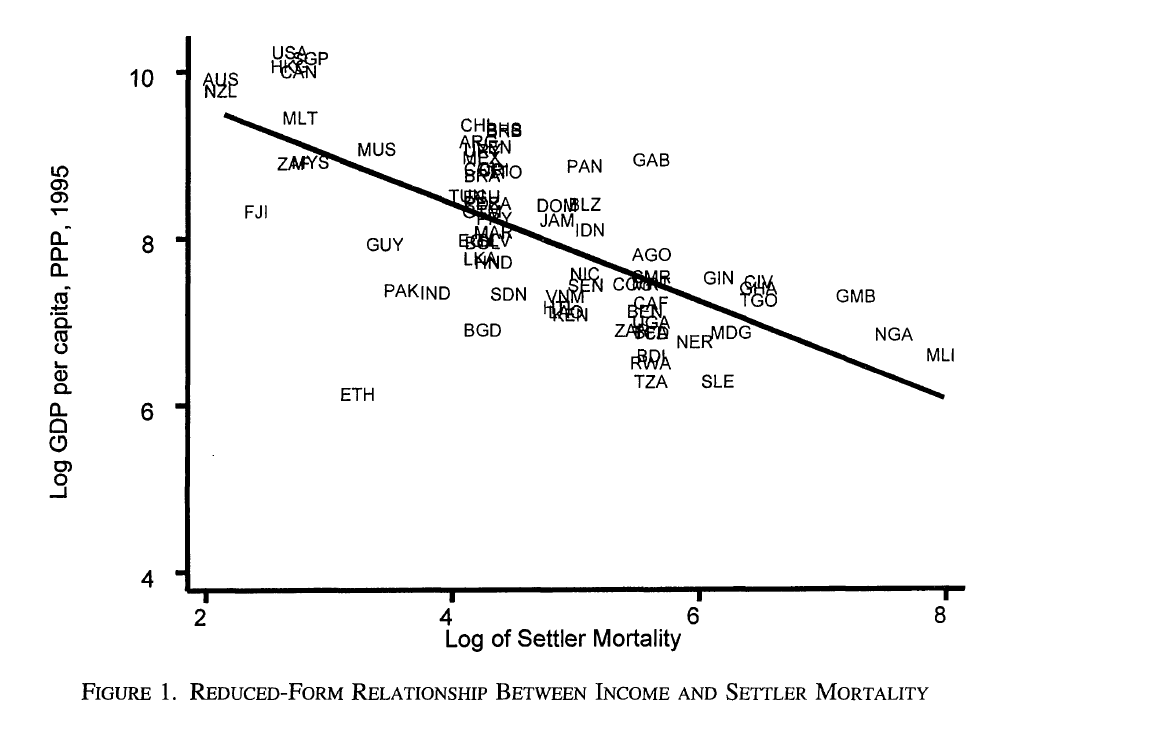
\includegraphics[scale=0.25]{Slides Principios de Economia/Figures/Magistral_09/M9.4.png} \vspace{2mm}
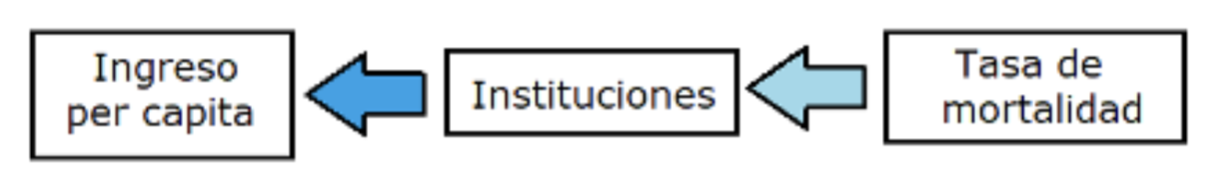
\includegraphics[scale=0.35]{Slides Principios de Economia/Figures/Magistral_09/M9.3.png} \\ \vspace{2mm}
\small Fuente: Acemoglu, Johnson \& Robinson (2001)
\end{frame}

\begin{frame}{Instituciones y eficiencia}
    \begin{itemize}
        \item Las instituciones afectan que tan eficiente (en el sentido de Pareto) son las asignaciones.
        \item Intituciones adecuadas nos pueden ayudar a alcanzar un equilibrio eficiente mientras que instituciones inadecuadas nos hacen caer en equilibrios ineficientes.
        \item Sin embargo, lo económico no necesariamente es el único objetivo de las instituciones.
        \item Conocer los criterios bajo los cuales una asignaión es justa o injusta es un problema de larga tradicion en filosofía y derecho.
    \end{itemize}
\end{frame}

\begin{frame}
\frametitle{Asignaciones y justicia}
\begin{itemize}
    \item Una asignación puede ser considerada justa o injusta en sí
    \begin{itemize}
        \item Un juicio substantivo de la justicia:
        \begin{itemize}
            \item Necesitamos una métrica de "lo que nos parece bien o mal"
            \item ¿Qué define que es justo?
        \end{itemize}
    \end{itemize}
    \item  Una asignación puede ser considerada justo o  injusta por la forma en que se llegó a ese resultado\vspace{2mm}
    \begin{itemize}
        \item Un juicio procedimental de la justicia
        \begin{itemize} 
            \item Necesitamos entender las reglas de juego y cómo se llegó al resultado 
            \item ¿Fueron los intercambios voluntarios?, ¿Fueron algunos individuos discriminados?, etc.
        \end{itemize}
    \end{itemize}
\end{itemize}
\end{frame}


\begin{frame}{Economía y justicia}
    \begin{itemize}
        \item Los valores que tiene la gente sobre lo que es justo y lo que no, varía entre individuos. ¿Podemos construir una teoría de la moral?
        \item El filósofo americano John Rawls sugirió como hacerlo:
        \begin{itemize}
            \item El velo de la ignorancia: imaginarse un tema sin saber qué lugar ocuparemos en esa sociedad (detrás del velo de la ignorancia)
            \item Elaboramos un juicio o evaluamos una institución desde atrás del velo.
            \item Por ejemplo: ¿los ricos deberían pagar más impuestos? ¿las personas con habilidades especiales deberían recibir una compensación del resto de la sociedad? 
          \end{itemize}
        \item La economía no hace juicios sobre lo que es justo o no, pero sí puede ayudarnos a pensar una serie de cosas: 
        \begin{itemize}
        \item Cómo las instituciones (reglas del juego) afectan las asignaciones y la desigualdad.
        \item Cómo explotar todas las situaciones de win-win que no generan conflicto.
        \item Qué tipo de políticas públicas son las mejores para lidiar con la injusticia
    \end{itemize}
    \end{itemize}
\end{frame}



\begin{frame}
\frametitle{Entendiendo el valor de las instituciones}
\begin{itemize}
    \item Vamos a visualizar el rol de las instituciones en la asignación de los recursos con un sencillo modelo. 
    \item Pensemos que existe un único trabajador y el factor productivo es la tierra (la propiedad de la tierra va a definir la nuestra discusión)
    \item Arrancamos con una frontera de posibilidades de producción 
        \begin{itemize}
        \item La frontera factible nos indica lo que es \textbf{tecnológicamente} posible, es decir, cuánto se puede producir cómo máximo en función de las horas de trabajo.
        \end{itemize}
    \item Pero ahora vamos a sumar una restricción que considera lo que es \textbf{biológicamente} posible.
        \begin{itemize} 
            \item Hay un mínimo de recursos que el individuo necesita para sobrevivir, aún si no produce nada...
            \item  ... y cuanta más energía utiliza produciendo, más recursos va a necesitar.
        \end{itemize}
    \end{itemize}
\end{frame}

\begin{frame}
\frametitle{La restricción biológica}
    \centering
    \begin{center}
    \begin{figure}[H]
    \renewcommand{\figurename}{Figure}
    \begin{center}
    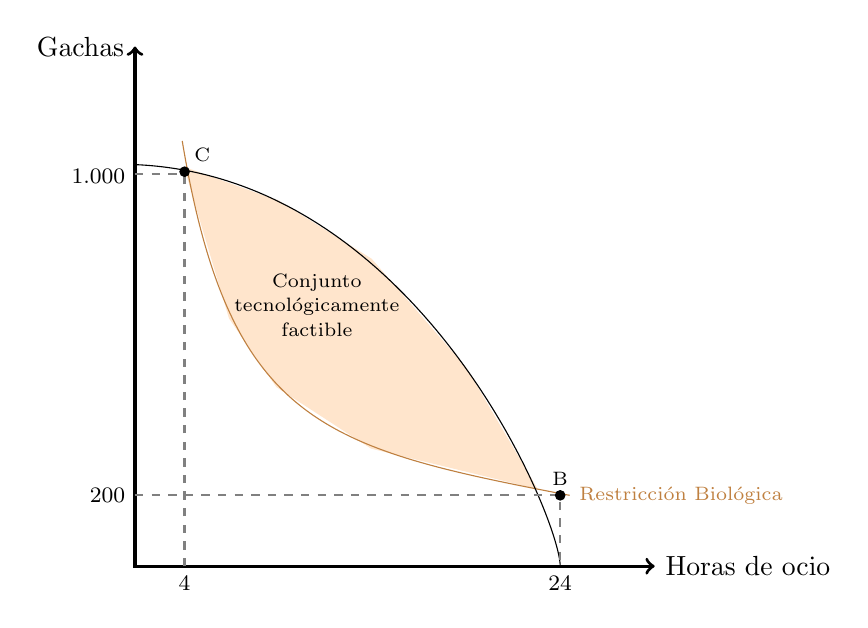
\begin{tikzpicture}[scale=0.6]
    \draw[fill,orange!20] (1.05,8.45)--(2,5.25)--(3,3.8)--(5,2.5)--(8.5,1.65)--(7,4.2)--(5,6.5)--(3,7.75);
    \draw[very thick,<->] (0,11) node[left]{Gachas}--(0,0)--(11,0) node[right]{Horas de ocio};
    \draw[thin, brown] (1,9).. controls (2,3) and (4, 2.5) .. (9.2, 1.5) node[right]{\scriptsize Restricción Biológica};
    \draw[thin] (0,8.5).. controls (6,8.25) and (9, 1) .. (9,0);
    \draw[thick, dashed, gray] (0,1.5)--(9,1.5)--(9,0);
    \draw[thick, dashed, gray] (1.05,0)--(1.05,8.25);
    \draw[thick, dashed, gray] (0,8.3)--(1.05,8.3);
    \node[below] at (1.05,0) {\footnotesize $4$};
    \node[below] at (9,0) {\footnotesize 24};
    \node[left] at (0,1.5) {\footnotesize $200$};
    \node[left] at (0,8.25) {\footnotesize $1.000$};
    \draw[fill] (9,1.5) circle [radius =0.1] node[above]{\scriptsize B};
    \draw[fill] (1.05,8.35) circle [radius =0.1] node[above right]{\scriptsize C};
    %\node[right] at (1,5) {\scriptsize Restricción Biológica};
    \node[] at (3.85,6) {\scriptsize Conjunto};
    \node[] at (3.85,5.5) {\scriptsize tecnológicamente};
    \node[] at (3.85,5) {\scriptsize factible};
    \end{tikzpicture}
    \end{center}
    \end{figure}
    \end{center}
\end{frame}


\begin{frame}{El objetivo es comparar distintas instituciones}
    Comparamos escenarios donde: \vspace{2mm}
        \begin{itemize}
            \item Situaciones históricas
            \begin{itemize}
                \item El régimen de esclavitud (Imperio Romano)
                \item Campesinos libres (EEUU en el siglo XVIII)
                \item Servidumbre con renta fija (Medioevo)
                \item Servidumbre con renta variable (Medioevo)
                \item La China comunista
                \item Un país con sindicatos\vspace{2mm}
            \end{itemize}
     \item ¿En qué forma queremos compararlas? Por ahora, en términos de eficiencia de Pareto
    \end{itemize}
\end{frame}


\begin{frame}
\frametitle{1. La esclavitud: ¿qué punto elige el amo?}
\begin{center}
\begin{figure}[H]
\renewcommand{\figurename}{Figure}
\begin{center}
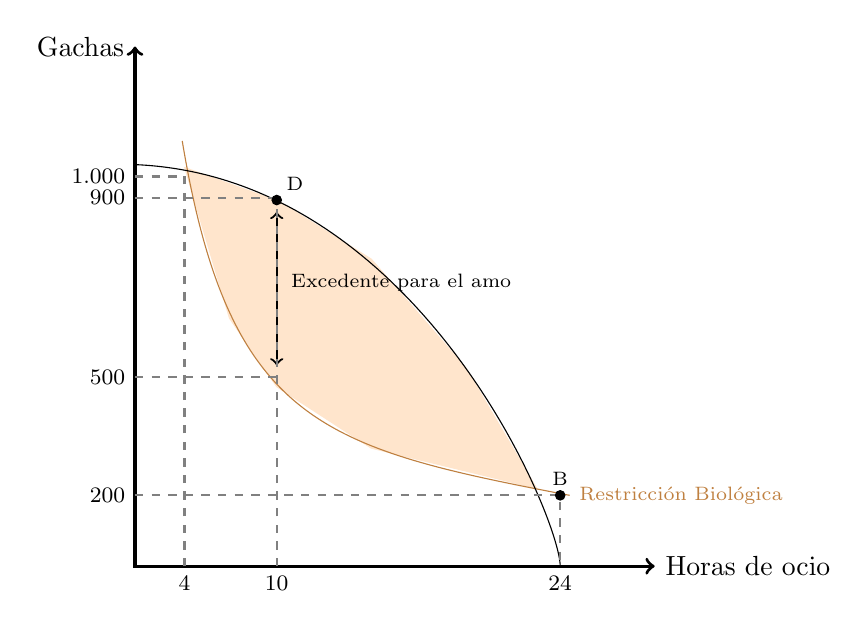
\begin{tikzpicture}[scale=0.6]
\draw[fill,orange!20] (1.05,8.45)--(2,5.25)--(3,3.8)--(5,2.5)--(8.5,1.65)--(7,4.2)--(5,6.5)--(3,7.75);
\draw[very thick,<->] (0,11) node[left]{Gachas}--(0,0)--(11,0) node[right]{Horas de ocio};
\draw[thin, brown] (1,9).. controls (2,3) and (4, 2.5) .. (9.2, 1.5) node[right]{\scriptsize Restricción Biológica};
\draw[thin] (0,8.5).. controls (6,8.25) and (9, 1) .. (9,0);
\draw[thick, dashed, gray] (0,1.5)--(9,1.5)--(9,0);
\draw[thick, dashed, gray] (1.05,0)--(1.05,8.25);
\draw[thick, dashed, gray] (0,8.25)--(1.05,8.25);
\node[below] at (1.05,0) {\footnotesize $4$};
\node[below] at (3,0) {\footnotesize $10$};
\node[below] at (9,0) {\footnotesize 24};
\node[left] at (0,1.5) {\footnotesize $200$};
\node[left] at (0,4) {\footnotesize $500$};
\node[left] at (0,8.25) {\footnotesize $1.000$};
\node[left] at (0,7.8) {\footnotesize $900$};
\draw[fill] (9,1.5) circle [radius =0.1] node[above]{\scriptsize B};
\draw[thick, <->] (3,4.25)--(3,7.5) ; 
\node[right] at (3.1,6) {\scriptsize Excedente para el amo};
\draw[thick, dashed, gray] (3,0)--(3,7.8);
\draw[thick, dashed, gray] (0,4)--(3,4);
\draw[thick, dashed, gray] (0,7.8)--(3,7.8);

\draw[fill] (3,7.75) circle [radius =0.1] node[above right]{\scriptsize D};
\end{tikzpicture}
\end{center}
\end{figure}
\end{center}
\end{frame}

\begin{frame}
\frametitle{1. La esclavitud: el equilibrio de la esclavitud}
\centering
\centering
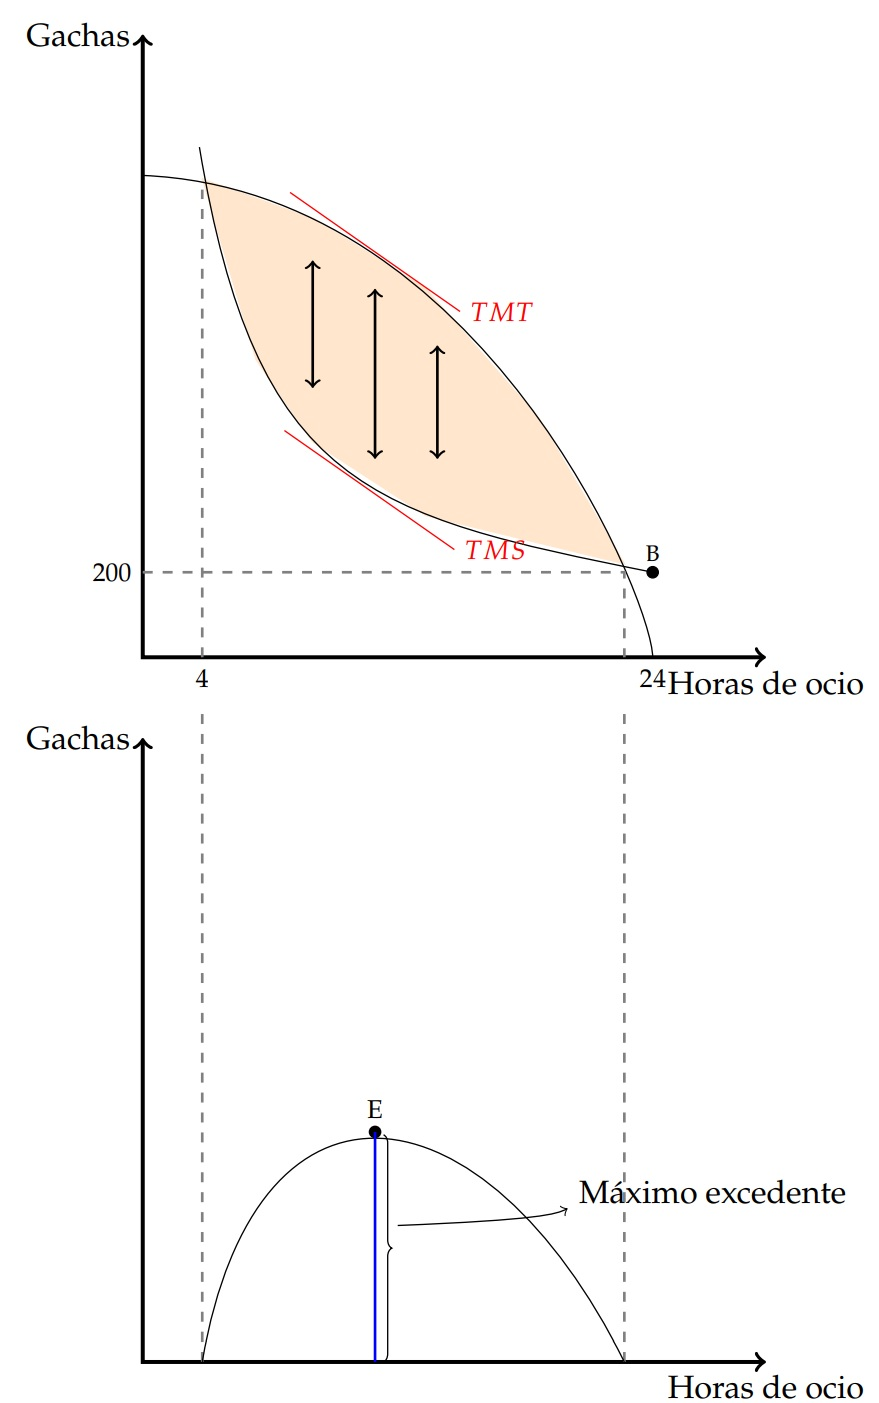
\includegraphics[scale=0.55]{Slides Principios de Economia/Figures/Magistral_09/C19.10.jpg}
\end{frame}

\begin{frame}
\frametitle{2. Ahora el esclavo se libera!}
        \begin{itemize}
            \item El trabajador podrá decidir libremente la cantidad de horas a trabajar.
            \item A diferencia de lo que sucedía con el caso del esclavo, ahora el trabajador va a tener en cuenta el costo del esfuerzo de su trabajo (la desutilidad del trabajo)  \vspace{1mm}
            \item Vamos a asumir que el trabajador, si no trabaja, tiene acceso a un monto mínimo que le permite vivir \vspace{1mm}
            \item Construimos la \textbf{curva de indiferencia de reserva del trabajador}. Esta curva de indiferencia nos indica todas las combinaciones de ocio y producto que le dan al agricultor la misma utilidad que su opción de reserva
            \begin{itemize}
                \item  Es decir, la curva de indiferencia incluye el costo de oportunidad de no trabajar.
            \end{itemize}
    \end{itemize}
\end{frame}

\begin{frame}
\frametitle{2. Ahora el esclavo se libera!}
\begin{center}
\begin{figure}[H]
\renewcommand{\figurename}{Figure}
\begin{center}
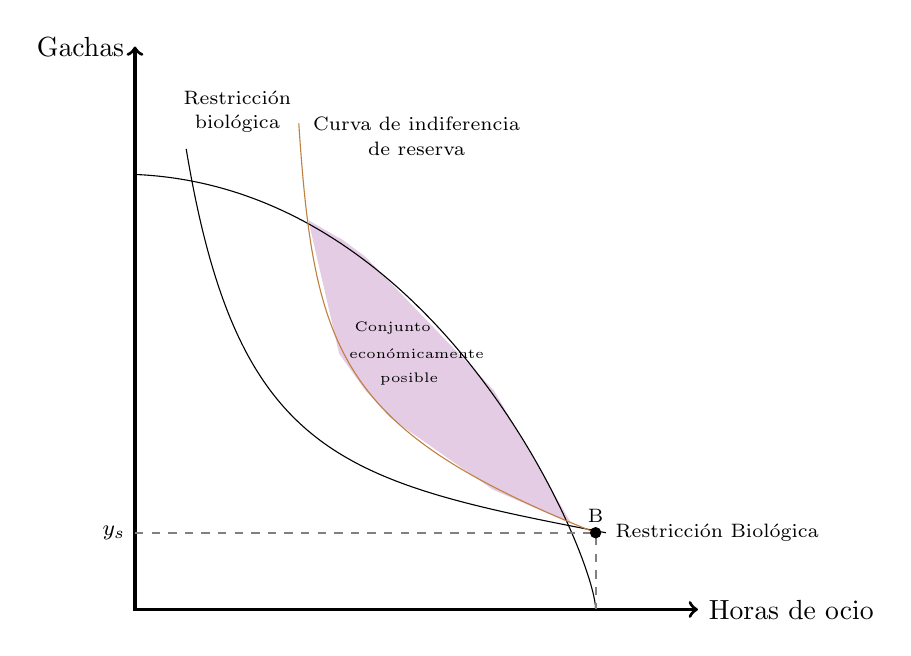
\begin{tikzpicture}[scale=0.65]
\draw[fill,violet!20] (3.4,7.6)--(4,5)--(4.5,4.3)--(5,3.75)--(7,2.35)--(8.5,1.7)--(7,4.28)--(4.5,6.88)--(4,7.25);
\draw[very thick,<->] (0,11) node[left]{Gachas}--(0,0)--(11,0) node[right]{Horas de ocio};
\draw[thin, black] (1,9).. controls (2,3) and (4, 2.5) .. (9.2, 1.5) node[right]{\scriptsize Restricción Biológica};
\draw[thin] (0,8.5).. controls (6,8.25) and (9, 1) .. (9,0);
\node[right] at (4.1,5.5) {\tiny Conjunto};
\node[right] at (4,5) {\tiny económicamente};
\node[right] at (4.6,4.5) {\tiny posible};
\draw[thin, brown] (3.2,9.5).. controls (3.5,5) and (4, 3.5) .. (9, 1.5);
\draw[thick, dashed, gray] (0,1.5)--(9,1.5)--(9,0);
\node[left] at (0,1.5) {\footnotesize $y_s$};

\draw[fill] (9,1.5) circle [radius =0.1] node[above]{\scriptsize B};
\node[] at (5.5,9.5) {\scriptsize Curva de indiferencia};
\node[] at (5.5,9) {\scriptsize  de reserva};
\node[] at (2,10) {\scriptsize Restricción};
\node[] at (2,9.5) {\scriptsize  biológica};
\end{tikzpicture}
\end{center}
\end{figure}
\end{center}
\end{frame}


\begin{frame}
\frametitle{2. La decisión del campesino libre}
\begin{center}
\begin{figure}[H]
\renewcommand{\figurename}{Figure}
\begin{center}
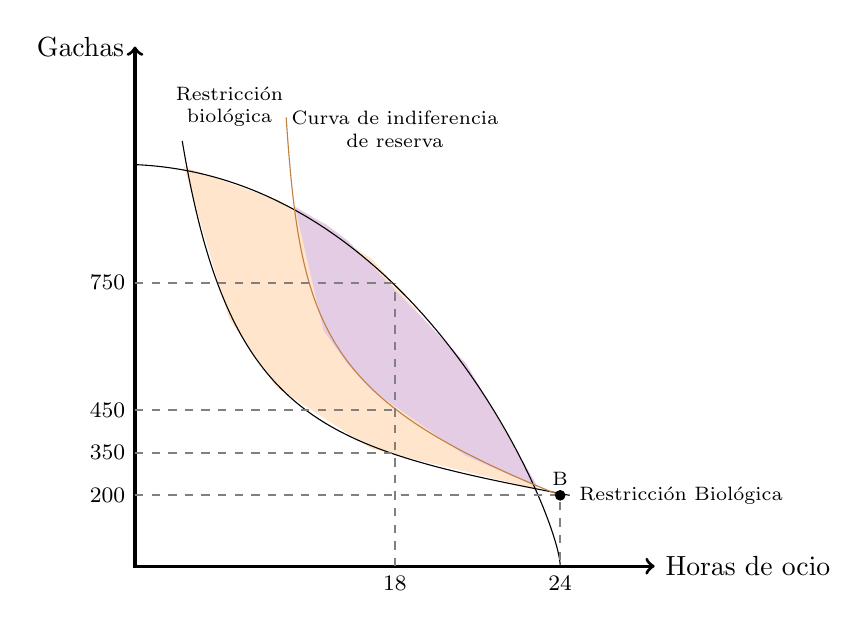
\begin{tikzpicture}[scale=0.6]
\draw[fill,orange!20] (1.05,8.45)--(2,5.25)--(3,3.8)--(5,2.5)--(8.5,1.65)--(7,4.2)--(5,6.5)--(3,7.75);
\draw[fill,violet!20] (3.4,7.6)--(4,5)--(4.5,4.3)--(5,3.75)--(7,2.35)--(8.5,1.7)--(7,4.28)--(4.5,6.88)--(4,7.25);
\draw[very thick,<->] (0,11) node[left]{Gachas}--(0,0)--(11,0) node[right]{Horas de ocio};
\draw[thin, black] (1,9).. controls (2,3) and (4, 2.5) .. (9.2, 1.5) node[right]{\scriptsize Restricción Biológica};
\draw[thin] (0,8.5).. controls (6,8.25) and (9, 1) .. (9,0);

\draw[thin, brown] (3.2,9.5).. controls (3.5,5) and (4, 3.5) .. (9, 1.5);
\draw[thick, dashed, gray] (0,1.5)--(9,1.5)--(9,0);
%\draw[thick, dashed, gray] (1.05,0)--(1.05,8.25);
%\draw[thick, dashed, gray] (0,8.25)--(1.05,8.25);
%\node[below] at (1.05,0) {\footnotesize $4$};
\node[below] at (5.5,0) {\footnotesize $18$};
\node[below] at (9,0) {\footnotesize 24};
\node[left] at (0,1.5) {\footnotesize $200$};
\node[left] at (0,2.4) {\footnotesize $350$};
\node[left] at (0,3.3) {\footnotesize $450$};
\node[left] at (0,6) {\footnotesize $750$};
%\node[left] at (0,8.25) {\footnotesize $1.000$};
%\node[left] at (0,7.8) {\footnotesize $900$};
\draw[fill] (9,1.5) circle [radius =0.1] node[above]{\scriptsize B};
%\draw[thick, <->] (3,4.25)--(3,7.5);
\draw[thick, dashed, gray] (5.5,0)--(5.5,6);
\draw[thick, dashed, gray] (0,6)--(5.5,6);
\draw[thick, dashed, gray] (0,3.3)--(5.5,3.3);
\draw[thick, dashed, gray] (0,2.4)--(5.5,2.4);
%\draw[thick, dashed, gray] (0,7.8)--(3,7.8);
\node[] at (5.5,9.5) {\scriptsize Curva de indiferencia};
\node[] at (5.5,9) {\scriptsize  de reserva};
\node[] at (2,10) {\scriptsize Restricción};
\node[] at (2,9.5) {\scriptsize  biológica};
%\node[] at (4.9,5.45) {\tiny Conjunto};
%\node[] at (5.2,5) {\tiny económicamente};
%\node[] at (5.5,4.55) {\tiny posible};

\end{tikzpicture}
\end{center}
\end{figure}
\end{center}
\end{frame}

\begin{frame}{Las diferencias entre la esclavitud y la libertad}
\centering
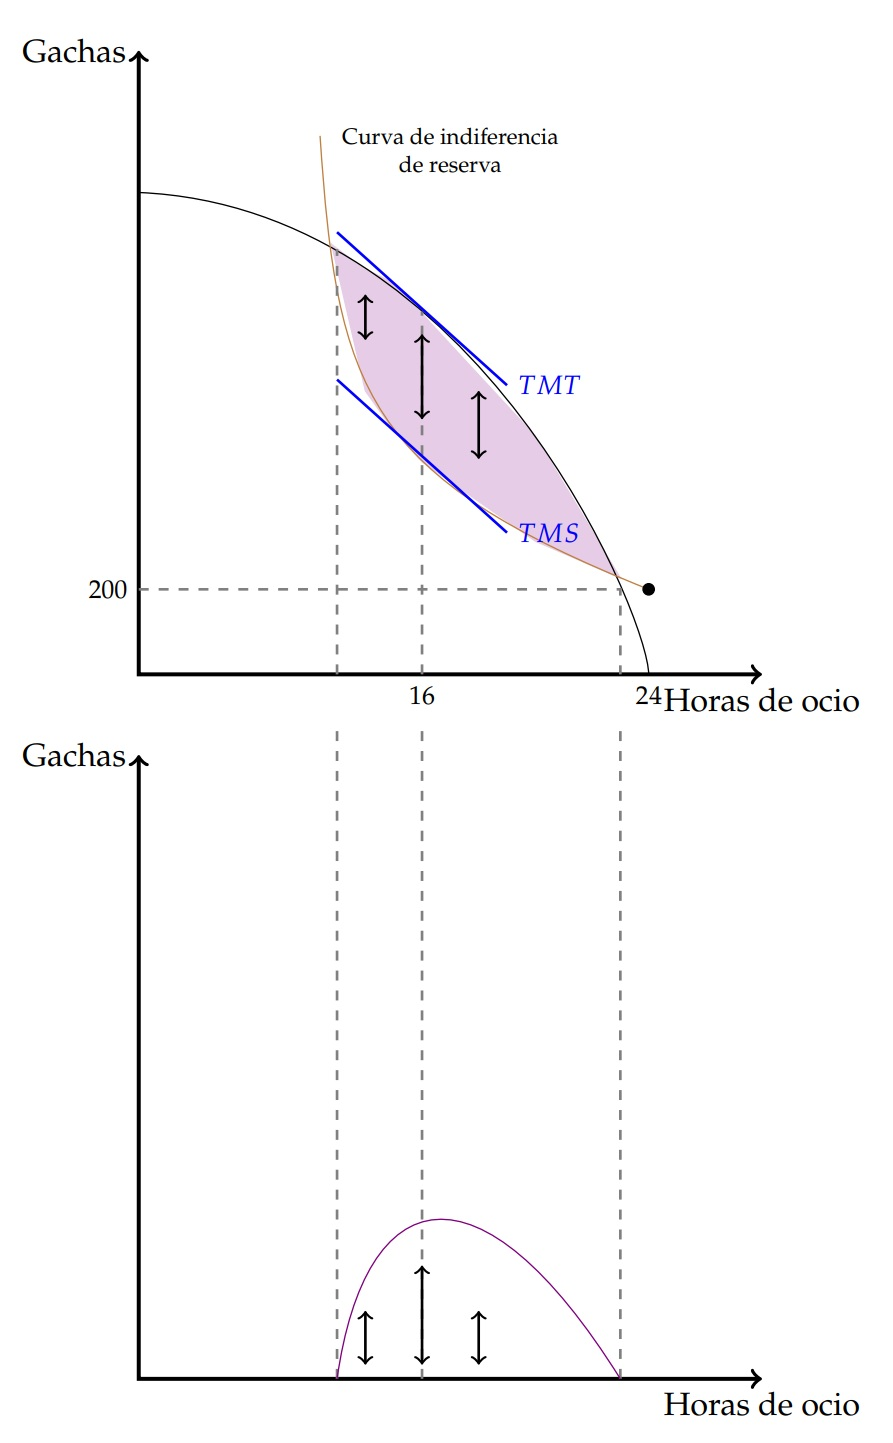
\includegraphics[scale=0.55]{Slides Principios de Economia/Figures/Magistral_09/C19.13.jpg}
\end{frame}

\begin{frame}{Las diferencias entre la esclavitud y la libertad}
        \begin{boxB}
        \centering
        En el óptimo, el trabajador elegirá el nivel de trabajo donde el costo marginal iguala a la producción marginal, que es el punto en el que se maximiza la diferencia entre estas dos curvas.
        \end{boxB}
        \begin{itemize}
        \item El punto máximo es cuando se iguala la pendiente de la curva de transformación con la de la curva de indiferencia de reserva. 
        \item El dueño de la tierra trabaja menos que en el régimen de esclavitud.
        \item Pero eso es óptimo: porque el régimen de esclavitud no tomaba en cuenta su desutilidad!
        \item El cambio de instituciones cambió la asignación (y la distribución).
    \end{itemize}
\end{frame}


\begin{frame}
\frametitle{3. Servidumbre medieval: servidumbre fija }
\begin{itemize}
    \item Estamos en la Edad Media donde un señor feudal es dueño de la tierra. 
    \item Se le permite a un campesino trabajar la tierra pero a cambio de una "arrendamiento". 
    \item  En este caso asumimos que el pago es un \textbf{monto fijo} de producción. \vspace{1mm}
    \item Para tomar la decisión de cuántas horas trabajar, el agricultor va a mirar la cantidad de producción que obtiene (por sobre su curva de indiferencia de reserva) luego de realizarle el pago al feudo \vspace{1mm}
        \begin{itemize}
        \item Tenemos que mirar la \textbf{nueva FPP} luego de pagar la renta
        \item Reduce lo que se lleva el campesino desplazando su retorno \textbf{paralelamente} hacia abajo. \vspace{1mm}
        \end{itemize}
    \item La producción no se modifica pero sí su distribución (ahora el campesino tiene que pasarle parte al señor feudal). 
\end{itemize}
\end{frame}

%\begin{frame}
%\frametitle{3. Servidumbre medieval: servidumbre fija }
%\centering
%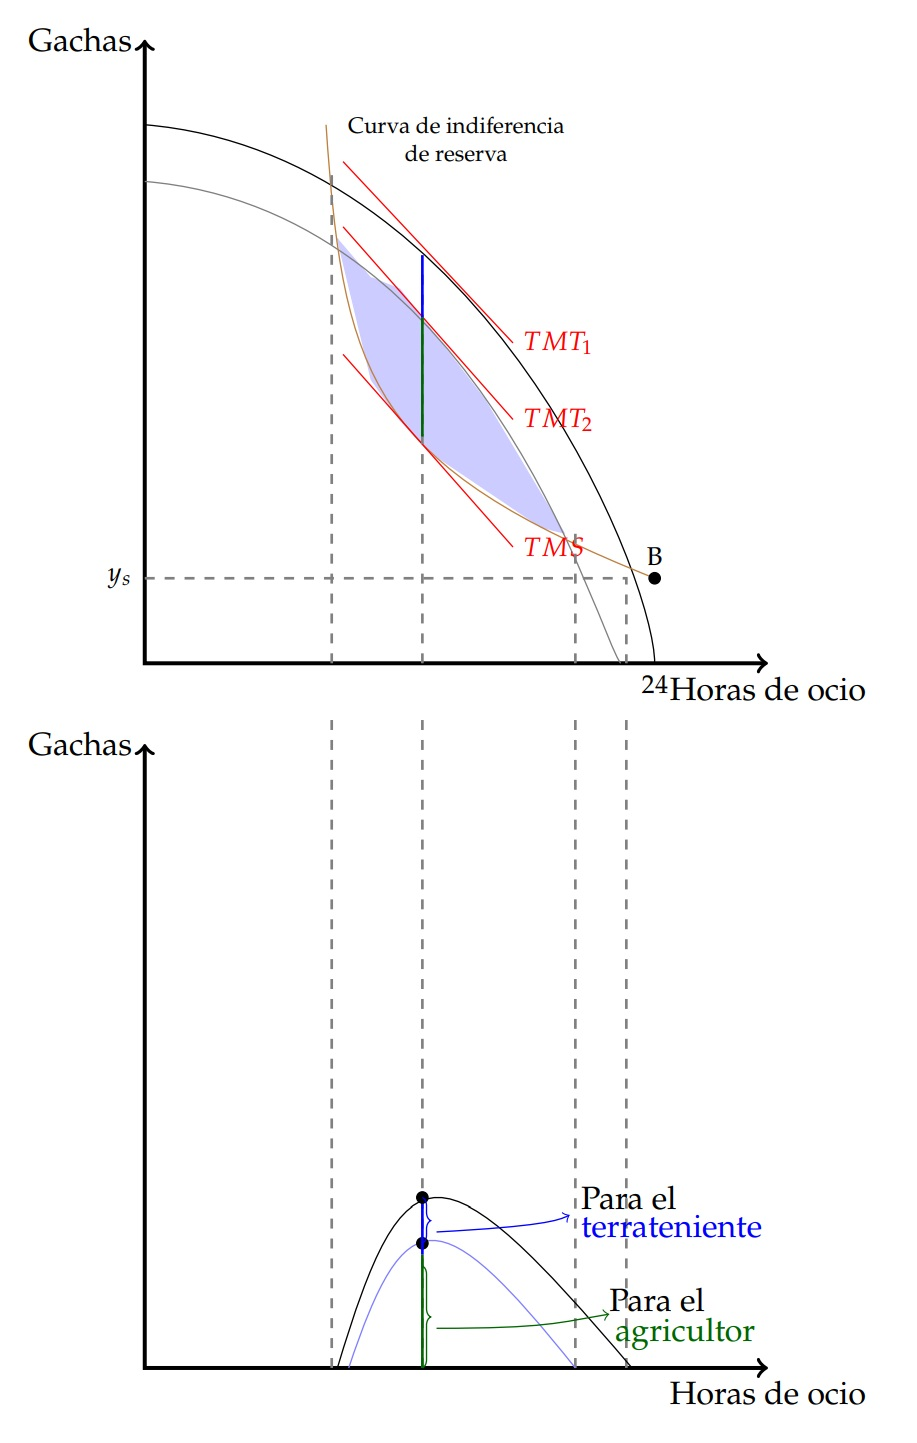
\includegraphics[scale=0.55]{Slides Principios de Economia/Figures/Magistral_09/C19.14.jpg}
%\end{frame}

\begin{frame}
\frametitle{3. Servidumbre medieval: servidumbre fija}

\begin{columns}
  \begin{column}{0.55\textwidth}
    \centering
    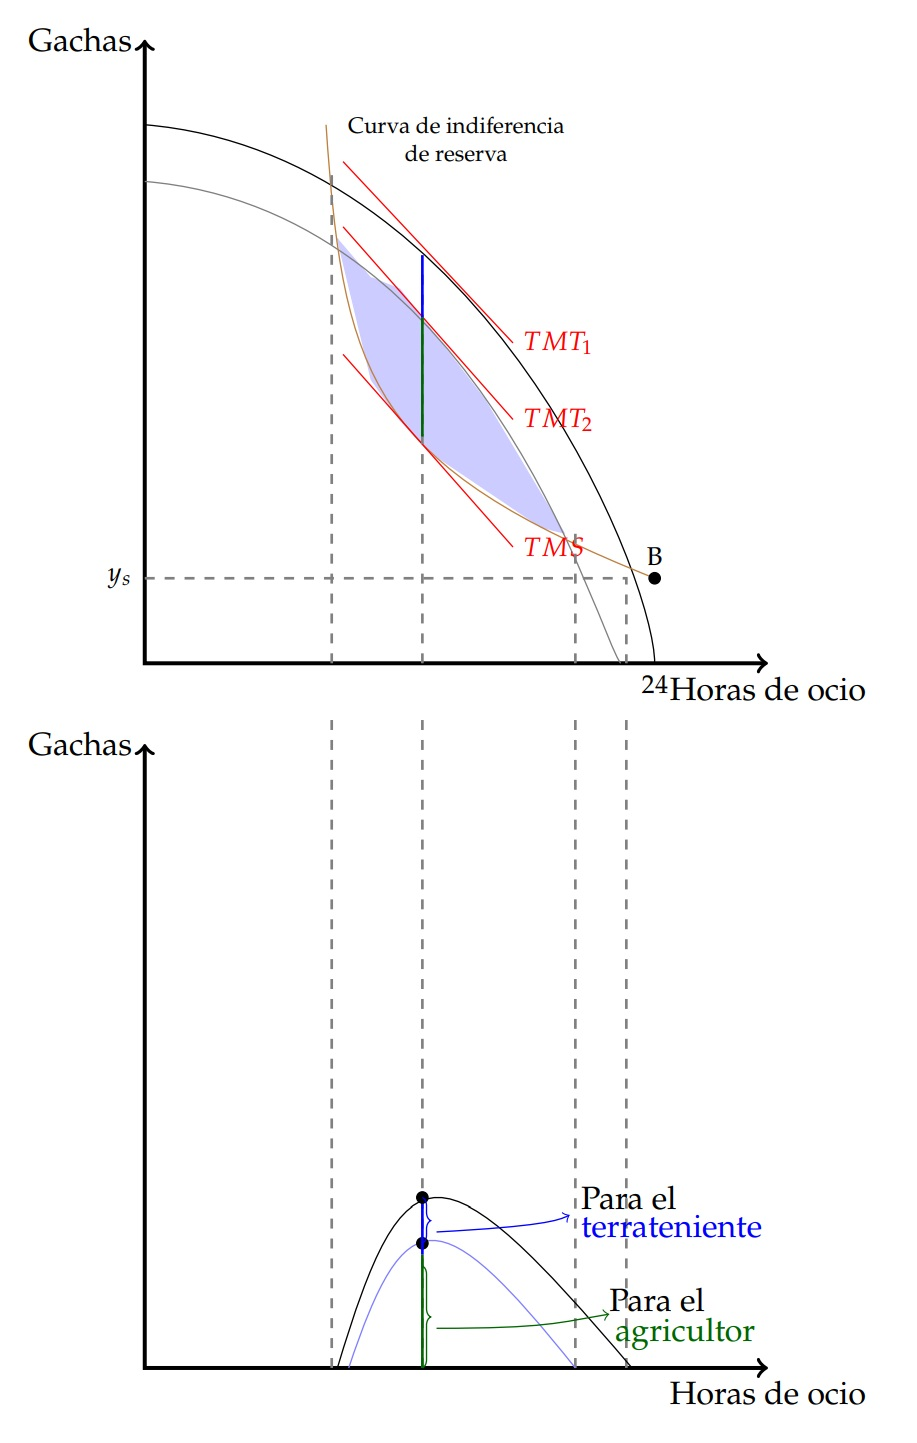
\includegraphics[scale=0.55]{Slides Principios de Economia/Figures/Magistral_09/C19.14.jpg}
  \end{column}

\begin{column}{0.45\textwidth}
    \begin{itemize}
        \item \small La pendiente de la FPP no se modifica
        \item \small El agricultor elige la misma cantidad de horas de trabajo que si fuese el dueño de la tierra    \item \small La diferencia es que, en el modelo donde el trabajador es dueño de la tierra, todo el excedente se lo quedaba el agricultor
        \item \small Llegamos a una situación eficiente
    \end{itemize}
  \end{column}
\end{columns}

\end{frame}

\begin{frame}
\frametitle{4. Servidumbre medieval: un porcentaje de la producción }
\begin{itemize}
    \item Ahora asumimos que el pago es un \textbf{porcentaje de la producción} $\rightarrow$ lo que se debe pagar al terrateniente aumenta a medida que aumenta la producción.
    \item Reduce lo que se lleva el campesino desplazando su retorno hacia abajo pero no de manera paralela sino que lo que se reduce crece con la producción
    \item La producción ahora cae respecto al caso anterior
     \item Hay una distorsión en la producción pero el riesgo está mejor distribuido entre el productor y el señor feudal. 
\end{itemize}
\end{frame}

\begin{frame}
\frametitle{4. Servidumbre medieval: un porcentaje de la producción}
\begin{columns}
  \begin{column}{0.55\textwidth}
    \centering
    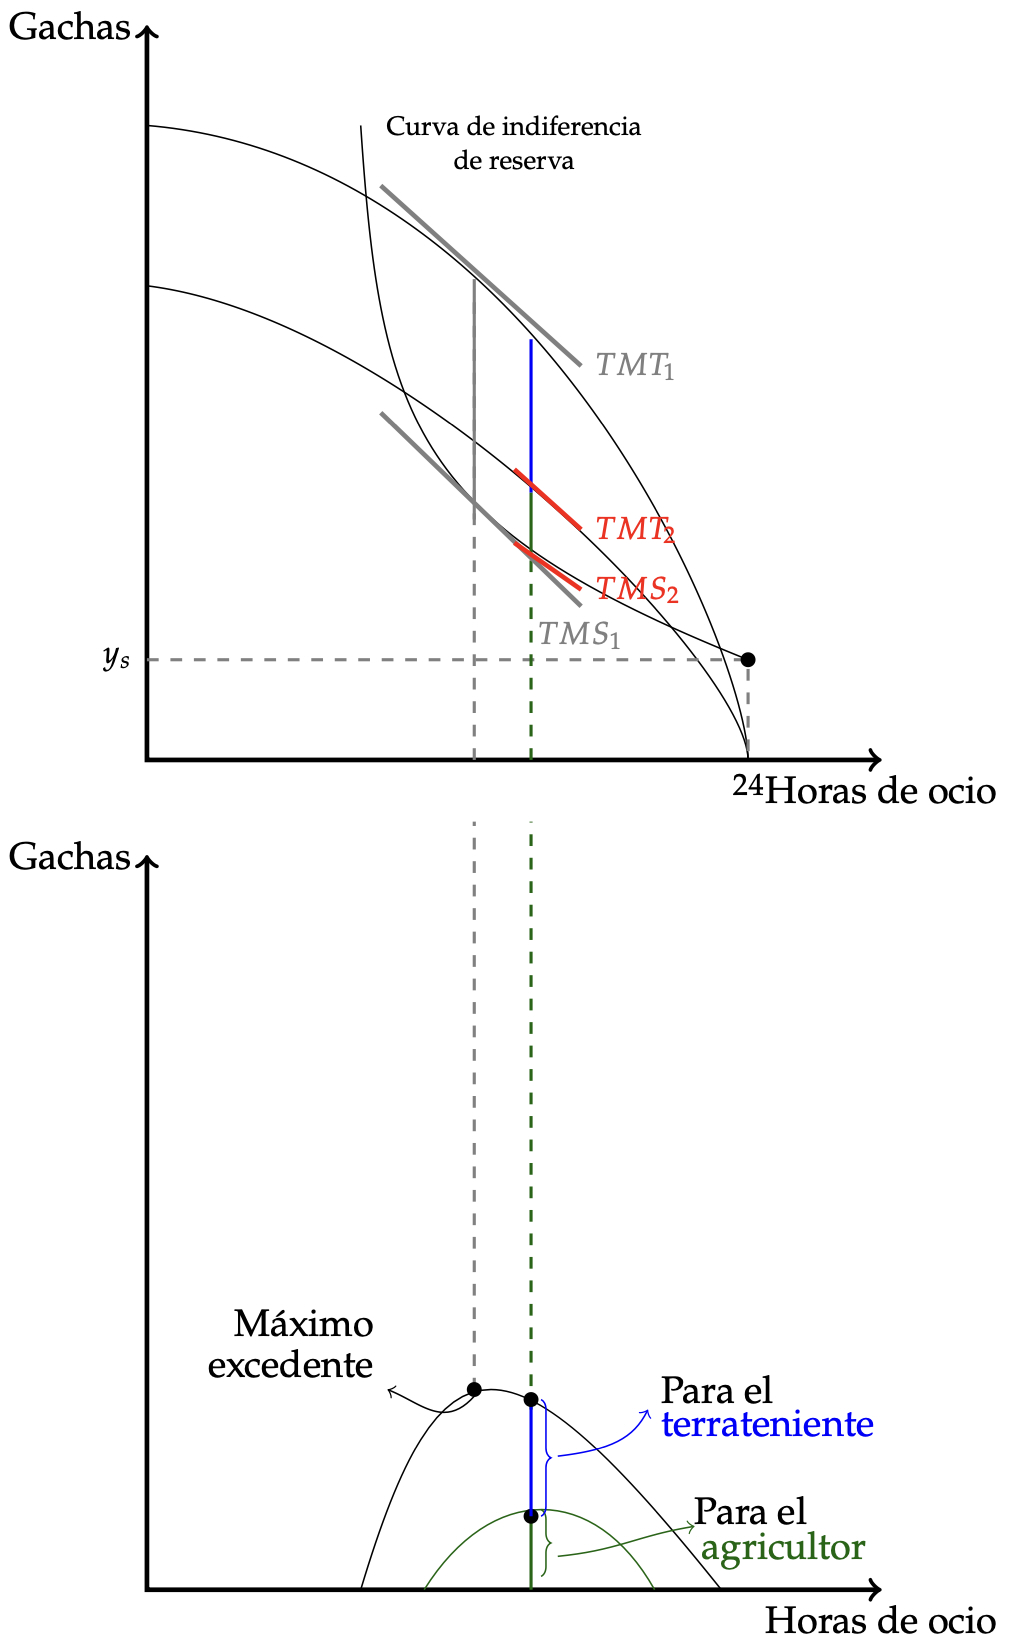
\includegraphics[scale=0.28]{Slides Principios de Economia/Figures/Magistral_09/C19.15.jpg}
  \end{column}

\begin{column}{0.45\textwidth}
    \begin{itemize}
        \item \small La pendiente de la FPP sí se modifica
        \item \small El ingreso marginal que logra el trabajador se reduce y esto reduce su incentivo a trabajar.
        \item \small El trabajador elige trabajar menos horas, en comparación a si fuese dueño de la tierra o si contrato es con monto fijo.
        \item \small Este contrato genera una asignación ineficiente
    \end{itemize}
  \end{column}
\end{columns}

\end{frame}


\begin{frame}
\frametitle{Diversificando riesgo en la Edad Media}
\centering
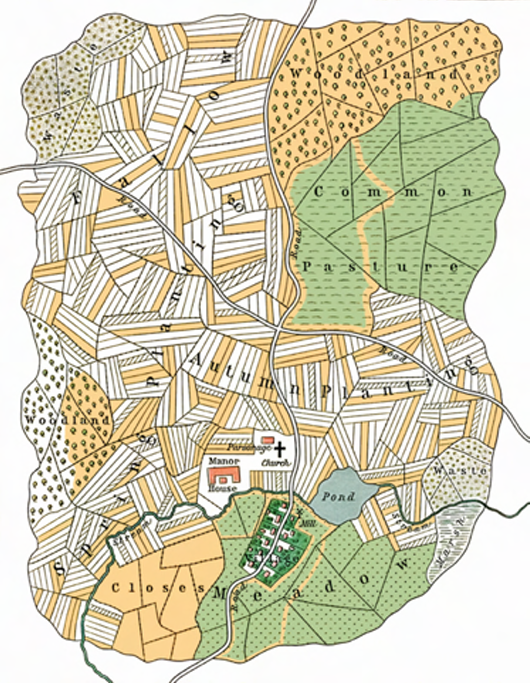
\includegraphics[scale=0.4]{Slides Principios de Economia/Figures/Magistral_09/C19.16.pdf}

\begin{itemize}
    \item Una manera de acotar el riesgo era partiendo las parcelas y distribuyéndolas en un área geográfica más amplia. 
\end{itemize}
\end{frame}

\begin{frame}
\frametitle{La China de Mao}
\begin{center}
\begin{figure}[H]
\renewcommand{\figurename}{Figure}
\begin{center}
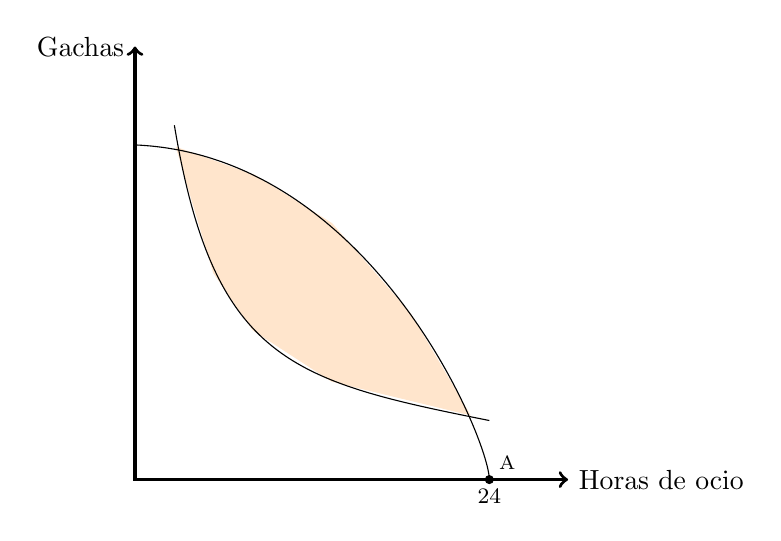
\begin{tikzpicture}[scale=0.5]
\draw[fill,orange!20] (1.05,8.45)--(2,5.25)--(3,3.8)--(5,2.5)--(8.5,1.65)--(7,4.2)--(5,6.5)--(3,7.75);
\draw[very thick,<->] (0,11) node[left]{Gachas}--(0,0)--(11,0) node[right]{Horas de ocio};
\draw[thin] (1,9).. controls (2,3) and (4, 2.5) .. (9, 1.5);
\draw[thin] (0,8.5).. controls (6,8.25) and (9, 1) .. (9,0);
%\draw[fill] (8.5,1.6) circle [radius =0.1] node[left]{$A$};
\draw[fill] (9,0) circle [radius =0.1];
%\draw[thick, <->] (4.5,0.15)--(4.5,4.35);
%\draw[thick, <->] (4.5,6.75)--(4.5,4.65);
\node[above right] at (9,0) {\scriptsize A};
%\node[] at (3.55,5.5) {\scriptsize dictador};
%\node[] at (3.5,2) {\scriptsize Para el};
%\node[] at (3.4,1.5) {\scriptsize productor};
\node[below] at (9,0) {\footnotesize 24};
%\node[below] at (8.5,0) {\footnotesize 23};
%\node[left] at (0,1.6) {\footnotesize 120 gr};
%\draw[thin, dashed, gray] (0,1.6)--(8.5,1.6);
%\draw[thin, dashed, gray] (8.5,0)--(8.5,1.6);
\end{tikzpicture}
\end{center}
\end{figure}
\end{center}
\begin{itemize}
\item Si siempre recibo lo mismo, sin importar la cantidad de trabajo, el óptimo está en el punto A donde el ocio es pleno y la producción es 0
    \end{itemize}
\end{frame}

\begin{frame}
\frametitle{La China de Mao }
\begin{itemize}
    \item Cuando Mao llega al poder decide la colectivización de las granjas
    \item Lo que recibe cada productor es independiente de lo que produce. 
    \item El productor maximiza su utilidad minimizando su trabajo 
     \item La producción baja a cero.  
     \item 40 millones de personas murieron de hambre
     \item ¡Vaya si las instituciones importan! 
\end{itemize}

\end{frame}

\begin{frame}
\frametitle{¿Qué pasa si hay un salario mínimo o un bono obligatorio?}
\centering
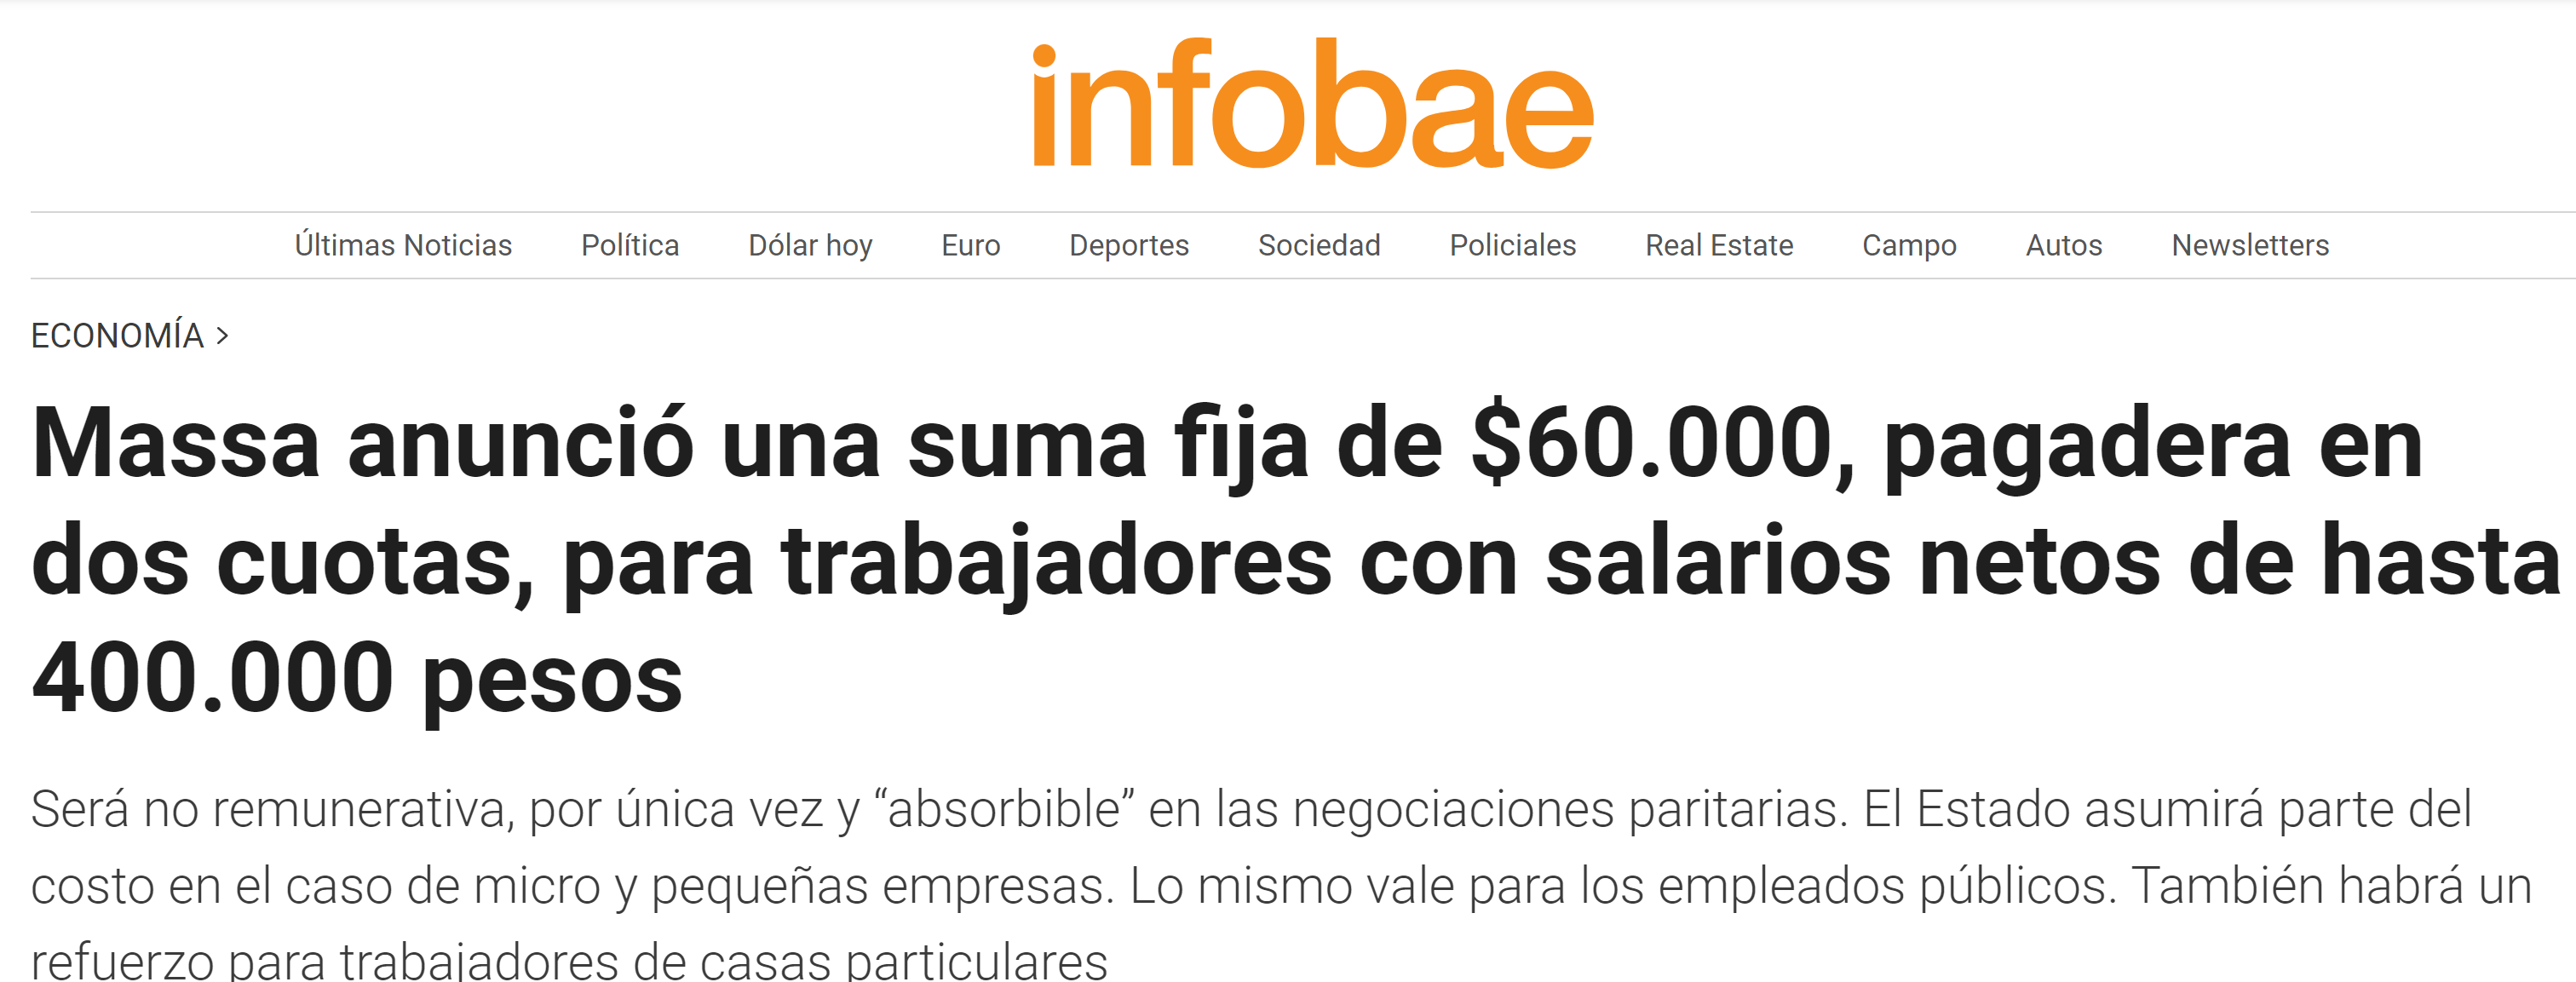
\includegraphics[scale=0.33]{Slides Principios de Economia/Figures/Magistral_09/M9.5.png}
\end{frame}

\begin{frame}
\frametitle{El gobierno sindical de Sudáfrica}
\begin{itemize}
    \item La remuneración de los trabajadores la define un "sindicato". 
    \item  Asumimos esa remuneración es mayor a la que ocurriría naturalmente
    \item Definido el salario, el dueño de la tierra define cuánto producir
    \item  La producción cae, pero la parte de la torta que se lleva el trabajador puede subir. 
\end{itemize}
\end{frame}

\begin{frame}
\frametitle{¿Qué pasa si hay un salario mínimo o un bono obligatorio?}
\centering
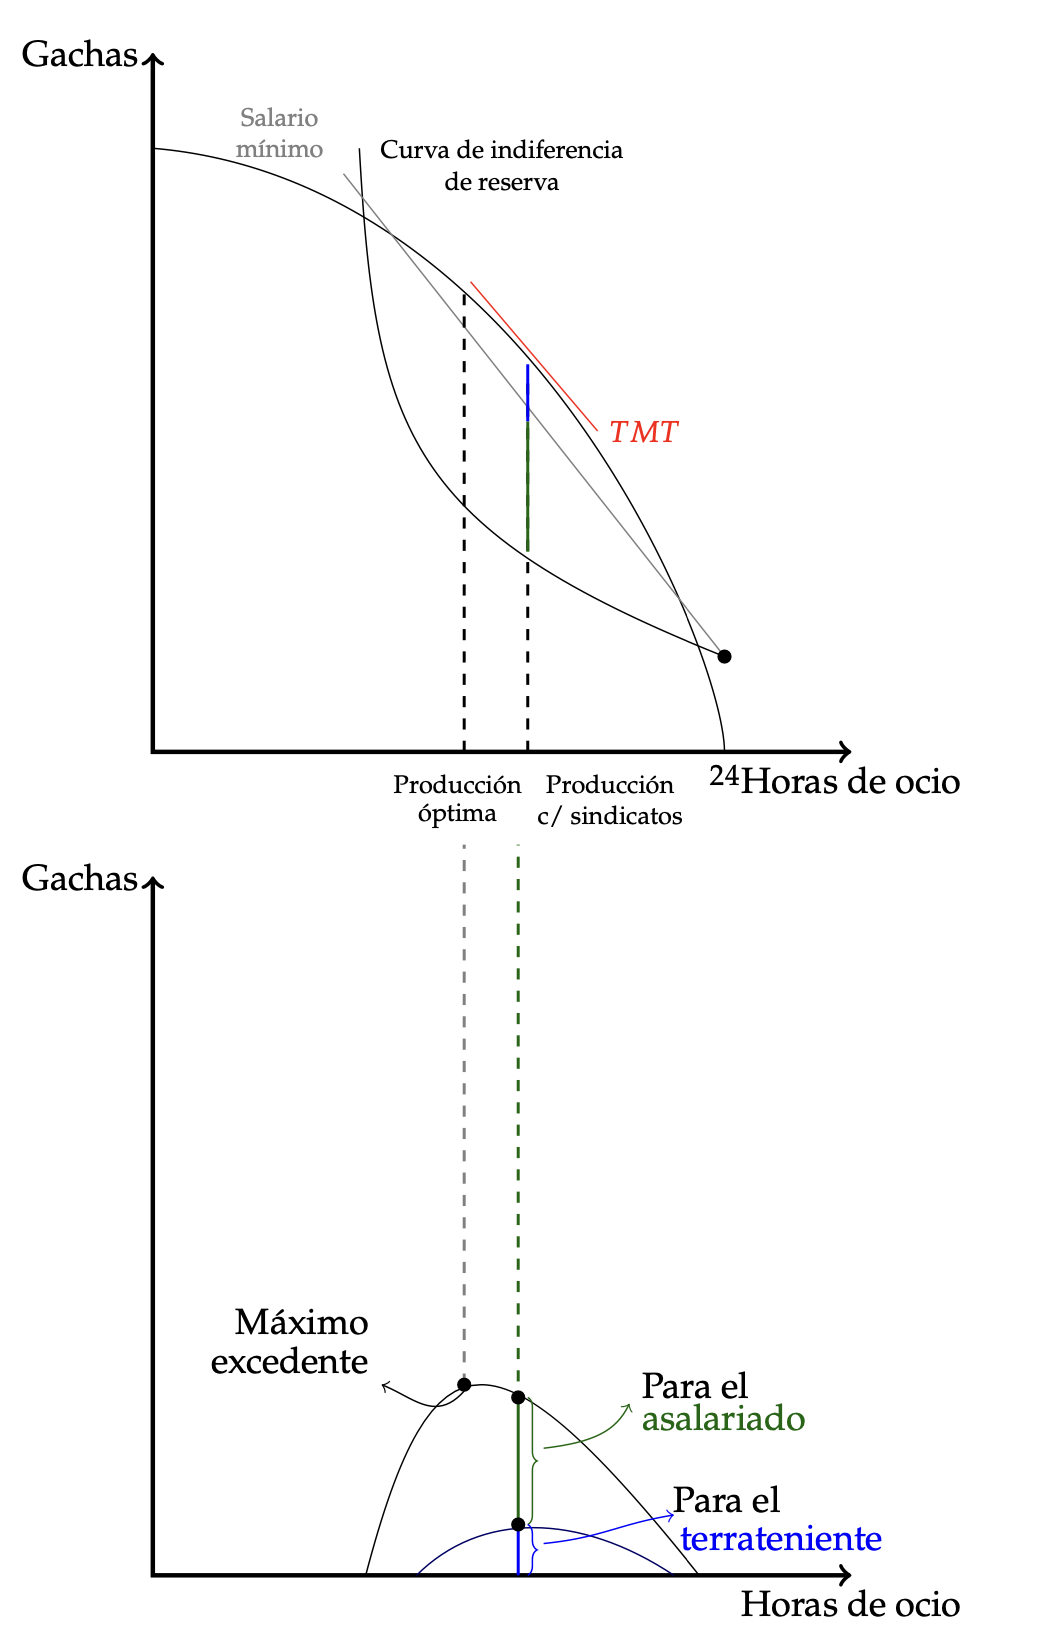
\includegraphics[scale=0.29]{Slides Principios de Economia/Figures/Magistral_09/C19.19.png}
\end{frame}

\begin{frame}
\frametitle{Conclusiones}
\begin{itemize}
    \item Las instituciones importan! \vspace{1mm}
    \item Las asignaciones económicas no solo dependen de las restricciones tecnológicas, biólogas y las preferencias, sino que también están condicionadas por las instituciones (tanto formales como informales) que limitan o afectan el conjunto viable de una situación.\vspace{1mm}
    \item Como los economistas pensamos en eficiencia,  querríamos evitar situaciones como la colectivización China o los contratos de arrendamiento que distorsionan la producción.
\end{itemize}
\end{frame}

\end{document}
